\setcounter{chapter}{4}
\chapter{Teoria delle Perturbazioni}

Fino a questo a momento abbiamo visto che per risolvere l'equazione di Schr\"odinger per un determinato sistema, \`e sufficiente determinare gli autovalori associati all'operatore Hamiltoniano. In particolare nei capitoli precedenti si \`e dimostrato come nel caso dell'atomo d'idrogeno e dell'oscillatore armonico sia possibile ottenere delle soluzioni analitiche esatte. Nella realt\`a non sempre si riesce a definire una soluzione esplicita del problema, per questo motivo si \`e ricercato dei \textit{metodi di approssimazione} che ci permettano di ottenere delle soluzioni analitiche approssimate del sistema di partenza in alcuni casi.

Il primo caso che andiamo a discutere \`e in riferimento alla perturbazione di una Hamiltoniana non esplicitamente dipendente dal tempo.


\section{Teoria delle perturbazioni indipendenti dal tempo}

Supponiamo  di avere una sistema quantistico descritto da un operatore Hamiltonianano $\hat{H}_0$ indipendente dal tempo i cui autostati sono $|\phi_n \rangle $ e autovalori $E_{n}^0$, ovvero
\begin{equation*}
	\hat{H}_0 |\phi_m \rangle = E_m^0 | \phi_{m} \rangle \quad m \in \mathbb{N}
\end{equation*} 
Assumiamo che gli autostati $\vert \phi_n \rangle$ formi una base ortonomale completa dello spazio degli stati
\begin{equation*}
	\langle \phi_{k} | \phi_m \rangle = \delta_{km}
\end{equation*}
inoltre lo spettro associato all'operatore \`e discreto, e gli autovalori di $\hat{H}_0$ non hanno degenerazione.

La teoria delle perturbazioni \`e applicabile quando abbiamo un sistema descritto da una Hamiltoniana che pu\`o essere scritta come
\begin{equation}
	\hat{H} =  \hat{H}_0 + \lambda \hat{V}
\end{equation}
dove $\hat{V}$ \`e un operatore Hermitiano e $\lambda \in \mathbb{R}$. La Hamiltoniana $\hat{H}_0$ descrive la fisica del sistema imperturbato e il termine $\lambda \hat{V}$ prendere il nome di \textit{perturbazione}. La grandezza del parametro $\lambda$  definisce l'intensit\`a della perturbazione che si applica al sistema.

Se la perturbazione che applichiamo al sistema \`e indipendente dal tempo questa prende il nome di \textit{perturbazione stazionaria}. Inoltre afficnh\`e gli elementi di $\lambda \hat{V}$ siano molto pi\`u piccoli di quelli dell'operatore $\hat{H}_0$, imponiamo la condizione che il termine $\lambda \ll 1$.

Lo scopo del metodo delle perturbazioni \`e quello di espandere gli autovalori e autostati di $\hat{H}$ in potenze di $\lambda$, mantenendo un numero finito di termini. Assumiamo l'esistenza di un intorno $\Lambda$ del punto $\lambda = 0$ dove per ogni $\lambda \in \Lambda$, la Hamiltoniana perturbata $\hat{H}$ ha un singolo autovalore non degenere $E_n(\lambda)$ con autostato associato $|\psi_n(\lambda) \rangle $. Inoltre assumi che per $\lambda \in \Lambda$ si ha che 
\begin{align*}
	& \lim_{\lambda \to 0}E_n(\lambda) = E_n^0 \\[0.5cm]
	& \lim_{\lambda \to 0} |\psi_{n}(\lambda) \rangle = |\phi_n \rangle 
\end{align*}
Per definizione abbiamo che $E_{n}(\lambda)$ e $|\psi_n(\lambda)\rangle$ soddisfano l'equazione 
\begin{equation}
	\hat{H}|\psi_n \rangle = E_n |\psi_n \rangle 
\end{equation}
in cui assumiamo tacitamente la dipendenza da $\lambda$. Definiamo lo stato $|\psi_n \rangle$ come combinazione lineare degli autostati $|\phi_n \rangle$ dell'operatore imperturbato $\hat{H}_0$.
\begin{equation}
	|\psi_n \rangle = \sum_{m} C_{mn}|\phi_m \rangle 
\end{equation} 
dove i coefficienti $C_{mn}(\lambda) = \langle \phi_m| \psi_n (\lambda) \rangle $. Sostituendo (5.3) in (5.2) e usando l'espressione (5.1) otteniamo la espressione
\begin{equation*}
	\sum_{m} (E_n - E_m^0)C_{mn}|\phi_{m} \rangle = \lambda \sum_{m} C_{mn}V|\phi_m \rangle 
\end{equation*} 
Moltiplicando l'equazione precedente da sinistra per $\langle \phi_k |$ abbiamo che
\begin{equation}
	(E_n - E_k^0) C_{kn} = \lambda \sum_{m} C_{mn} \langle \phi_k|V|\phi_m \rangle  = \lambda \sum_{m}V_{km}C_{mn}
\end{equation} 
dove $V_{km} \equiv \langle \phi_k|V|\phi_m \rangle $. Vogliamo ora risolvere (5.4) rispetto ai coefficienti $C_{kn}(\lambda)$ e gli autovalori $E_{n}(\lambda)$. In particolare vogliamo trovare una soluzione perturbata rispetto ai termini di espansione $\lambda$. Dato che la funzione $| \psi_n(\lambda) \rangle $ \`e analitica per $\lambda \in \Lambda$, possiamo espandere i termine $C_{nm}(\lambda)$ come serie di potenze di $\lambda$:
\begin{equation}
\begin{array}{l}
C_{mn} ( \lambda)   = \langle \phi_m|\psi_n(\lambda) \rangle = \\[0.5cm]
 = \langle \phi_m | \Big( |\phi_n \rangle + \lambda |\psi_n^1 \rangle + \lambda^2|\psi_n ^2 \rangle + ... \Big ) = \\[0.5cm]
 = \delta_{nm} + \lambda \langle \phi_m|\psi_{n}^2 \rangle +  \lambda^2 \langle \phi_m| \psi_n^2 \rangle + ... = \\[0.5cm]
 \equiv \delta_{mn} + \lambda C_{mn}^1 + \lambda^2 C_{nm}^2 + ....   
\end{array}
\end{equation}
Dalla relazione (5.3) abbiamo che 
\begin{equation}
	|\psi_n ( \lambda) \rangle = |\phi_n \rangle + \lambda \sum_{m} C_{mn}^1|\phi_m \rangle + \lambda^2 \sum_{m} C_{mn}^2|\phi_m \rangle + ...
\end{equation}
Se $\lambda = 0$ l'equazione (5.4) si riduce alla condizione 
\begin{equation*}
	(E_n^0 - E_k^0)\delta_{kn} = 0
\end{equation*} 
Se $\lambda \neq 0$ e $\lambda \in \Lambda$, possiamo espandere gli autovalori $E_n(\lambda)$ in serie di potente di $\lambda$ nel seguente modo:
\begin{equation}
	E_n(\lambda) =\sum_{\alpha = 0}^{\infty} \lambda^\alpha E_{n}^{\alpha} = E_{n}^0 + \lambda E_n^1 + \lambda^2 E_n^2 + ... 
\end{equation}
Notare che per i termini $C_{nm}^\alpha$ e $E_n^\alpha$ gli esponenti sono solo nomenclature e non rappresentano delle potenze come nel caso di $\lambda$.

Sostituendo nell'equazione (5.4) per $\lambda = 0$  gli elementi (5.5) e (5.7) per poi raccogliere i termini con la stessa potenza in $\lambda$, otteniamo 
\begin{align}
	0  = & \delta_{kn} (E_n^0 - E_k^0) +  \notag \\[0.5cm] 
		& + \lambda \Big [ \delta_{kn}E_{n}^1 + C^1_{kn}(E^0_n-E_k^0) -V_{kn} \Big] + \notag \\[0.5cm]
		& + \lambda^2 \Big [ \delta_{kn}E^2_{n} + C^2_{kn}(E_n^0 - E_{k}^0) + C_{kn}^1E_n^1 - \sum_{m}V_{km}C_{mn}^1 \Big] + ...
\end{align}
di conseguenza tutti i coefficienti rispetto a $\lambda$ devono essere nulli. Il primo termine \`e automaticamente 0 per definizione. 

\subsection{Correzioni al primo ordine $\mathcal{O}(\lambda)$}

I coefficienti al primo ordine $\mathcal{O}(\lambda)$ sono nulli quando
\begin{align}
	& E_n^1 = V_{nn} \quad \quad \quad\quad k = n \\[0.5cm]
	& C_{kn}^1 = \frac{V_{kn}}{E^0_n - E^0_k} \quad \;k \neq n
\end{align}
Chiaramente notiamo che $C_{nn}^1$ non \`e determinabile dall'equazione (5.8).  Se moltiplichiamo l'equazione (5.1) ambo i lati per una costante Z arbitraria modifichiamo la norma di $|\psi_n \rangle$, ma non l'autovalore associato $E_n$
\begin{equation*}
	\hat{H}(Z|\psi_n \rangle) = E_n (Z|\psi_n \rangle)
\end{equation*}
questo ci dice che siamo libere di scegliere il valore di $\langle \psi_n | \psi_n \rangle $. Scegliamo di normalizzare $|\psi_n \rangle$ in modo tale che: 
\begin{equation}
	\langle \phi_n | \psi_n \rangle = 1
\end{equation}
Sostituendo (5.3) in (5.11) abbiamo che 
\begin{equation*}
	C_{nn}( \lambda) = 1
\end{equation*} 
e quindi usando la relazione (5.5) avremo la seguente equazione
\begin{equation}
	1 = C_{nn}(\lambda) = 1 + \lambda C_{nn}^1 + \lambda^2 C_{nn}^2 + ...
\end{equation}
di conseguenza affinch\`e l'identit\`a sia verificata dobbiamo avere che per i coefficienti per ogni potenza di $\lambda$ siano nulli  
\begin{equation}
	C^{\alpha}_{nn} = 0 \quad \alpha \in \mathbb{N}
\end{equation}
In conclusione possiamo riassumere i risultati ottenuti per le perturbazioni al primo ordine nel seguente modo:
\begin{align}
	& E_n( \lambda) = E_n^0 + \lambda \langle \phi_n | \hat{V} | \phi_n \rangle + ... \\[0.5cm]
	|\psi_n(\lambda) \rangle &= |\phi_n \rangle + \lambda \sum_{k \neq m} C_{kn}^1|\phi_k 
	\rangle + ... \notag \\[0.5cm]
	& = |\phi_n \rangle  + \lambda \sum_{k \neq n} \frac{\langle \phi_k|\hat{V}|\phi_n \rangle}{E_n^0-E_k^0}|\phi_k \rangle + ...
\end{align}
Queste due espressioni rendono chiaro il significato di "piccole perturbazioni". Dobbiamo avere che 
\begin{equation*}
	\langle \phi_n| \lambda \hat{V}|\phi_n \rangle \ll E_n^0
\end{equation*}
e
\begin{equation*}
	| \langle \phi_k| \lambda \hat{V} | \phi_n \rangle | \ll |E_n^0 - E_k^0|
\end{equation*}
Se le due condizioni non vengono rispettate, l'espansione ottenuta non \`e una buona approssimazione degli autovalori ed autostati della Hamiltoniana associata al sistema perturbato.

 L'espressione (5.15) ci dice che le correzioni al primo ordine degli autostati sono una serie infinita che dipende dagli elementi matriciali della perturbazione $\hat{V}$.
 
\subsection{ Correzioni al secondo ordine $\mathcal{O}(\lambda^2)$}

Consideriamo i termini al secondo ordine in $\lambda$. Il fatto che i coefficienti in $\lambda^2$ siano nulli ci porta ade avere le seguenti relazioni
\begin{align}
	& E_n^2 = \sum_{m} V_{nm}C_{mn}^1 - C^1_{nn}E_n^1  \quad \quad \quad k = n\\[0.3cm]
	& C^2_{kn} = \frac{1}{E_n^0-E_k^0} \Big( \sum_{m} V_{km}C_{mn}^1 - C_{kn}^1E_n^1 \Big  ) 
	\quad \quad \quad  k \neq n
\end{align}  
Usando i risultati (5.9),(5.10) e (5.13) le espressioni precedenti possono essere riscritte nel seguente modo:
\newpage 
\begin{align}
	& E_n^2 = \sum_{m \neq n} \frac{|V_{nm}|^2}{E_n^0-E_m^0} \quad \quad \quad k = n \\[0.3cm]
	& C^2_{kn} = \frac{1}{E_n^0 - E_k^9} \left( \sum_{m \neq n} \frac{V_{km}V_{mn}}{E_n^0-E_m^0} - \frac{V_{kn}V_{nn}}{E_n^0-E_k^0} \right) \quad \quad \quad k \neq n
\end{align}
Per scrivere (5.21) abbiamo usato il risultato che $V_{mn} = (V_{nm})^*$ dato che $\hat{V}$ \`e per ipotesi \`e un operatore autoaggiunto.
Utilizzando i risultati ottenuti fino a questo punto possiamo riscrivere i termini di grado pi\`u basso come 
\begin{align}
E_n^1 & =\left\langle\phi_n\right| \hat{V}\left|\phi_n\right\rangle \\[0.3cm]
\left|\psi_n^1\right\rangle & =\sum_{k \neq n} \frac{\left\langle\phi_k\right| \hat{V}\left|\phi_n\right\rangle}{E_n^0-E_k^0}\left|\phi_k\right\rangle \\[0.3cm]
E_n^2 & =\sum_{k \neq n} \frac{\left|\langle\phi_n | \hat{V}| \phi_k\rangle \right|^ 2}{E_n^0-E_k^0}
\end{align}

\begin{wrapfigure}{r}{0.4\textwidth} % 'r' for right, 'l' for left
    \centering
    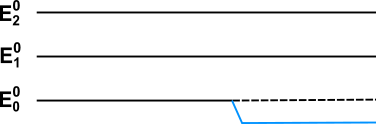
\includegraphics[width=0.37\textwidth]{energystate} % Replace with your image file
    \label{fig:example}
\end{wrapfigure}
Se un sistema di trova al livello fondamentale $E_0^0$ nell'equazione (5.22) si ha a denominatore una grandezza $(E_0^0-E_m^0) < 0$ dato che  l'energia $E_0^0$ \`e il minimo valore che il sistema pu\`o assumere. 
In generale dalle perturbazioni al secondo ordine il livello fondamentale viene sempre abbassato.

\begin{wrapfigure}{l}{0.4\textwidth} % 'r' for right, 'l' for left
    \centering
    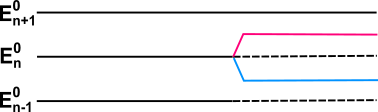
\includegraphics[width=0.37\textwidth]{energystate1} % Replace with your image file
    \label{fig:example}
\end{wrapfigure}
Per uno stato generico n-simo, si ah che per $n > m$ la perturbazione innalza il livello energetico, mentre per $m > n$ lo abbassa. Se sono presenti grandi spazi energetici tra i vari livelli si ha un contributo perturbativo minore rispetto a quelli pi\`u ravvicinati.

\subsection{Il coefficiente $C_{nn}^1$}

Per determinare il coefficiente $C^{1}_{nn}$ nella precedente sezione abbiamo scelto una normalizzazione dello stato $|\psi_n \rangle$ affinch\`e valesse la condizione (5.11). Inoltre tacitamente si \`e assunto che i termini fossero dei numeri reali, in realt\`a quando calcoliamo i coefficienti l'espressione (5.12) dovrebbe considerare il fatto che gli addendi $C_{nn}^{1}$ possono essere numeri complessi
\begin{align}
	1 & = \langle \psi_n| \psi_n \rangle = (\langle \phi_n| + \lambda \langle \psi_n|^1 +...)(|\phi_n \rangle + \lambda |\psi_n \rangle^1 +...) = \notag \\& = 1 +\lambda \langle \psi_n|^1\phi_n \rangle + \lambda \langle \phi_n|\psi_n \rangle^1 +... )=1 + \lambda(C^{1*}_{nn} + C_{nn}^1)+...
\end{align} 
 di conseguenza
 \begin{equation}
  C_{nn}^{1*} + C_{nn}^1 = 0
 \end{equation}
che equivale al sistema di equazioni

\begin{equation}
	\left \{ \begin{array}{l}
		Re(C_{nn}^1) = 0 \\[0.3cm]
		C_{nn}^1 = i\theta \quad \theta \in \mathbb{R}
	\end{array} \right.
\end{equation}
Dunque riscrivendo l'espansione dello stato $|\psi_n \rangle$ rispetto ai risultati in (5.17) abbiamo che
\begin{align*}
	|\psi_n \rangle & = | \phi_n \rangle  + \lambda (C_{nn}^1 | \psi_n \rangle + \sum_{m \neq n}C_{nm}^1 |\phi_m \rangle +...)+... = \\[0.5cm]
	& =(1+ \lambda C_{nn}^1)|\phi_n \rangle + \lambda\sum_{m \neq n}C_{nm}^1 |\phi_m \rangle +...)+... =   
\end{align*}
il termine $1+ \lambda C_{nn}^1 = 1 + \lambda i \theta$ coincide con lo sviluppo di Taylor arrestato al primo ordine della funzione $e^{i\lambda \theta}$ e quindi l'espressione precedente diventa
\begin{equation*}
	= e^{i \lambda \theta} (|\phi_n \rangle  + \lambda \sum_{m \neq n}C_{nm}^1|\psi_m \rangle +.. ) + ...
\end{equation*}
quindi abbiamo dimostrato che $C_{nn}^1$ non \`e necessariamente un termine nullo, ma pu\`o coincidere con un numero complesso di modulo unitario, che introduce un termine di fase che in meccanica quantistica pu\`o essere considerato trascurabile.

\section{Teoria delle perturbazioni indipendenti dal tempo degeneri}

Il problema \`e il medesimo di quello trattato nella sezione precedente solo che in questo caso assumiamo che i livelli energetici ammettano degenerazione.
Da un punto di vista qualitativo se $E_n^0$ \`e un autovalore degenere ci aspettiamo che i livelli reali siano sovrapposti e che l'introduzione di una perturbazione li separi.

Assumiamo che lo stato $E_n^0$ associato al sistema imperturbato possieda una degenerazione di  grado $g$; questo vuol dire che esiste un insieme di dimensione $g$ di autostati associati allo stesso autovalore.
\begin{equation}
	 \{ |\phi_n \rangle, |\phi_{n^1} \rangle, ....,|\phi_{n^g} \rangle \} 
\end{equation}
tutti associati al medesimo autovalore $E^0_{D}$,
\begin{equation*}
	E_n^0 = E_{n^1}^0 = \ldots =E_{n^g}^0 \equiv E_{D}^0
\end{equation*}
In questo caso a priori non possiamo imporre la condizione che 
\begin{equation}
	\lim_{\lambda \to 0 } |\psi_n \rangle = |\phi_n \rangle 
\end{equation}
siccome non sappiamo a quali valori dell'insieme (5.26) la funzione di stato $|\psi_n \rangle $ va a coincidere al ridursi del coefficiente perturbativo. Potrebbe anche convergere ad una loro combinazione lineare 
\begin{equation}
|\varphi\rangle=\left\langle\phi_n \mid \varphi\right\rangle\left|\phi_n\right\rangle+\left\langle\phi_{n^{\prime}} \mid \varphi\right\rangle\left|\phi_{n^{\prime}}\right\rangle+\ldots+\left\langle\phi_{n^{\prime \prime \ldots \prime \prime}}\mid \varphi\right\rangle\left|\phi_{n^{\prime \prime\ldots \prime \prime}}\right\rangle
\end{equation}
al tendere $\lambda \to 0 $. 
Data questa ambiguit\`a possiamo anche definire l'equazione del sistema senza indici
\begin{equation*}
	\hat{H}(\lambda)|\psi(\lambda) \rangle = E(\lambda)|\psi(\lambda) \rangle
\end{equation*}
ed espandiamo lo stato $|\psi \rangle $ rispetto alla base $\{|\phi_k \rangle \}$ isolando esplicitamente i contributi dati dagli stati degeneri associati al medesimo autovalore $E_{D}^0$
\begin{equation}
	|\psi(\lambda) \rangle = \sum_{m \in D} C_{m}(\lambda)|\phi_m \rangle + \sum_{k \not \in D}C_k(\lambda)|\phi_k \rangle
\end{equation}
dove $D = \{1,\ldots,g \}$ fa riferimento agli indici che identificano gli autostati degeneri.
Imponiamo la condizione per cui 
\begin{equation}
\lim_{\lambda \to 0} \equiv |\psi^0 \rangle = |\varphi \rangle 	
\end{equation}
dove, per definizione
\begin{equation}
	|\varphi \rangle = \sum_{m \in D} \langle \phi_m | \varphi \rangle |\phi_m \rangle  \quad \text{e} \quad \langle \varphi \mid \varphi \rangle = 1
\end{equation}
Dell'espressione (5.31) esistono almeno $g$ combinazioni lineari indipendenti possibili. Posto $\lambda = 0$ e utilizzando il risultato (5.30) abbiamo che l'equazione (5.29) assume la forma 
\begin{align}
	|\psi^0 \rangle & = \sum_{m \in D}C_{m}^0|\phi_m \rangle + \sum_{k \not \in D}C_{k}^0|\phi_k \rangle = \notag \\[0.5cm]
	& =  \sum_{m \in D} \langle \phi_m | \varphi \rangle |\phi_{m} \rangle 
\end{align}
dove abbiamo definito $C_{m}^0 \equiv C_m(\lambda = 0)$. Tale risultato ci dice che 
\begin{equation*}
	C_{k}^0 = \left \{ \begin{array}{l}
		\langle \phi_k|\varphi \rangle \quad k \in D \\[0.3cm]
		0 \quad \quad \quad \; k \not \in D
	\end{array}\right.
\end{equation*}
Ora procediamo come nel caso non degenere. Innanzitutto abbiamo che 
\begin{equation}
	(E - E_k^0) C_k = \lambda \sum_{m} V_{km}C_{m}
\end{equation}
Espandendo in serie di potenze coefficienti ed energie abbiamo 
\begin{equation*}
	C_k(\lambda) = C_k^0 + \lambda C_{k}^2 + \lambda^2 C_{k}^2 + \ldots 
\end{equation*}
 e
 \begin{equation*}
 	E(\lambda) = E_{D}^0 + \lambda E^1 + \lambda^2 E^2 + \ldots 
 \end{equation*}
 Sostituendo le due equazioni in (5.33) e raccogliendo i termini associati alla stessa potenza, abbiamo che 
 \begin{align}
0 & =  C_k^0\left(E_D^0-E_k^0\right) \notag \\[0.5cm]
& +\lambda\left[C_k^0 E^1+C_k^1\left(E_D^0-E_k^0\right)-\sum_m V_{k m} C_m^0\right] \notag \\[0.5cm]
& +\lambda^2\left[C_k^0 E^2+C_k^2\left(E_D^0-E_k^0\right)+C_k^1 E^1-\sum_m V_{k m} C_m^1\right]+\ldots
\end{align}
I coefficienti per ogni potenza di $\lambda$ devono essere nulli. 

\subsection{Correzioni al primo ordine $\mathcal{O}(\lambda)$}
Al primo ordine abbiamo che i coefficienti sono nulli quando valgono le seguenti condizioni 
\begin{align}
	& \sum_{m \in D} V_{km} \langle \phi_m|\varphi \rangle = E^1 \langle \phi_k| \varphi \rangle \quad \quad \;\; k \in D \\[0.5cm]
	& C_k^1(E_D^0-E_k^0) = \sum_{m \in D} V_{km} \langle \phi_{m} | \varphi \rangle \quad  k \not \in D
\end{align}
Chiaramente, le grandezze $V_{km}$ con $k,m \in D$, possono essere interpretate come elementi di una matrice $g \times g$. La relazione (5.35) pu\`o essere vista come un equazione rispetto agli autovalori che determina i $g$ autovalori $\{ E_{a}^2 \} = \{ E_{1}^1,E_{2}^2,...,E_{g}^1\} $ e i corrispondenti $g$ autostati $\{|\varphi_a \rangle  \} = \{ |\varphi_1 \rangle, |\varphi_2 \rangle ,...,|\varphi_g \rangle \} $. L'equazione (5.35) implica che in presenza di una perturbazione del sistema, l'insieme dei $g$ autostati degeneri $|\phi_n \rangle , |\phi_{n'} \rangle, \ldots , |\phi_{n^{'' \ldots ''}} \rangle  $ con autovalori $E_{D}^0$, vengono trasformati rispetto al primo ordine in un nuovo insieme di autostati $|\varphi_{1} \rangle, \ldots | \varphi_{g} \rangle $ con autovalori $E_{D}^0 + \lambda E_{1}^1,E_{D}^0 + \lambda E_{2}^1, \ldots,E_{D}^0 + \lambda E_{g}^1$.
Assumendo che i nuovi autovalori sia non degeneri, possiamo dire che \textit{la perturbazione ha rimosso la degenerazione}.

\section{Effetto Stark - Atomo d'idrogeno in un campo elettrico costante}

In questa sezione studiamo l'effetto Stark nell'idrogeno come esempio di teoria delle perturbazioni per uno stato legato. L'effetto Stark riguarda il comportamento degli atomi in presenza di un campo elettrico costante. 

Le prime osservazioni della divisione delle linee spettrali di un atomo per via dell'interazione con un campo elettrico sono state fatte da Stark nel 1913, che gli valse il premio Nobel nel 1919.
\newpage

\subsection{Sistema imperturbato}

Abbiamo un sistema costituito da un nucleo attorno al quale orbita un solo elettrone, ignorando lo spin delle particele, vogliamo studiare lo stato fondamentale dell'atomo d'idrogeno.

L'atomo a singolo elettrone viene modellato usando la Hamiltoniana che esprime un sistema a forza centrale 
\begin{equation}
	\hat{H}_0 = \frac{p^2}{2m} + V_0(r)
\end{equation}
dove per l'idrogeno abbiamo che
\begin{equation*}
	V_0 (r) = - \frac{e^2}{r}
\end{equation*}
Prima di iniziare a descrivere il sistema perturbato, abbiamo bisogno di capire il comportamento di quello imperturbato, a partire dalle sue energie, autostati e degenerazioni. Nel modello elettrostatico, i livelli di energia del sistema imperturbato sono descritti dalla formula Bohr
\begin{equation*}
	E_n = - \frac{1}{2n^2}\frac{e^2}{a_0} = -\frac{E_0}{n^2} \quad n \in \mathbb{N}
\end{equation*}
dove il termine $a_0$ indica il raggio di Bohr ed $E_0 = 13,6 \; eV$ l'energia associata allo stato fondamentale. Per l'atomo d'idrogeno gli atuovalori hanno una degenerazione di $n^2$. Gli autostati associati sono dati da 
\begin{equation*}
	|nlm \rangle = \psi_{nlm}(\bold{x}) = R_{nl}Y_{lm}(\theta,\phi)
\end{equation*}
dove le funzioni $Y_{lm}(\theta, \phi)$ sono armoniche sferiche.

\subsection{Potenziale}
Scriviamo la forza esterna $\bold{F}$ dovuta al campo elettrico esterno ed assumiamo che abbia orientazione lungo l'asse $\hat{u}_{z}$,
\begin{equation*}
	\bold{F} = F \hat{u}_{z}
\end{equation*}
Di conseguenza il potenziale della perturbazione ha forma
\begin{equation*}
	V_1 = q \phi = - q\bold{F} \cdot \bold{x} = eFz
\end{equation*}
dove si \`e considerato $q = -e $. Il potenziale imperturbato $V_0$ dipende da $r$, mentre quello perturbato $V_1$ dipende da $z$, di conseguenza abbiamo che la perturbazione del sistema rompe la simmetria di rotazione $SO(3)$ presente nel sistema imperturbato.

\subsection{Effetto Stark nello stato fondamentale}

Iniziamo la trattazione nel caso del sistema perturbato partendo dallo stato fondamentale dell'atomo di idrogeno; in notazione chimica coincide con la configurazione $1s$ che corrisponde all'autostato $| 100\rangle $. Siccome allo stato fondamentale non \`e presente degenerazione la correzione di energia al prima ordine \`e data da 
\begin{equation*}
	E^1_{0} = \langle 100|V |100 \rangle = 0 
\end{equation*}
che risulta essere nulla poich\`e 
\begin{equation*}
	\langle 100| eEz | 100 \rangle = eE \langle 100|z|100 \rangle  = eE\frac{1}{4 \pi} \int_{-\infty}^{\infty}dz z = 0 
\end{equation*}
dato che $z$ \`e una funzione dispari. Quindi possiamo concludere che al primo ordine per lo stato fondamentale dell'idrogeno non \`e presente una perturbazione al primo ordine dell'energia e di conseguenza nessun effetto Stark.
Osserviamo per\`o che  esiste una perturbazione del secondo ordine dello stato fondamentale, determinando
\begin{equation*}
	E_p^{(2)} = \sum_{q \neq p} \frac{|\langle \phi_q|V|\phi_p \rangle |^2}{(E_p^0-E_q^0)} = \sum_{nlm \neq 100} \frac{\langle nlm | eEz|100 \rangle|^2}{E_0/n^2-E_0} < 0
\end{equation*}
e quindi il livello $1s$ dell'atomo d'idrogeno viene abbassato di un ordine $\mathcal{O}(E^2)$. Resta comunque valida l'osservazione che non esista nessun effetto Stark per l'atomo d'idrogeno al livello fondamentale dato che questo coinvolge solo le perturbazioni del primo ordine delle energie.
\subsection{Effetto Stark negli stati eccitati dell'idrogeno}

Gli stati eccitati dell'idrogeno per $n \geq 2$ hanno una degenerazione tra gli stati con opposta parti\`a, dato che $l = 0,...,n-1$ e la parti\`a \`e pari per $l$ parti e dispari per $l$ dispari.  In accordo con la teoria descritta in precedenza per le perturbazioni di secondo ordine, la variazione dei livelli di energia $E_n$ \`e data dagli autovalori della matrice $n^2 \times n^2$, indicizzata da $(lm)$ e $(l'm')$
\begin{equation*}
	\langle nlm| eFz|nl'm' \rangle 
\end{equation*}
La matrice che si ottiene \`e di grandi dimensioni, ma molti elementi risultano essere nulli per motivi di simmetria. Consideriamo come esempio il caso per $n = 2 $. Abbiamo quattro stati degeneri inclusi nei livelli $2s$ con autostati $|nlm \rangle = |200 \rangle $ e il livello $2p$ con autostati $|21m \rangle $ con $m = 0, \pm 1$. 

Otterremo una matrice di  dimensione $4 \times 4$ i cui elementi si calcolano usando la relazione  $\langle \phi_i|V|\phi_j \rangle $ con $\phi_i = \{ \underbrace{ |211 \rangle, |21-1\rangle ,|210 \rangle }_{2p}, \underbrace{|200 \rangle}_{2s} \}$. Complessivamente la matrice possiede 16 elementi, per evitare di calcolarli tutti possiamo riassumerli sinteticamente nel seguente modo
\begin{equation*}
	\langle 200|z|200 \rangle  \sim \int_{-\infty}^{+\infty}dz  \; z = 0
\end{equation*}
per parit\`a della funzione $z$. 
\begin{equation*}
	\langle 21m|z|21m'\rangle \sim \int_{- \infty} ^{+ \infty}d\bold{x} \; Y_{1m}^*zY_{1m'} = 0 \quad m' \neq 0
\end{equation*}
gli elementi sono nulli per parit\`a. Gli unici termini non nulli della matrice sono dati da 
\begin{equation*}
	\langle 21m|z|200 \rangle \sim \int_{\mathbb{R}^3} d\theta() \int_{0}^{2\pi} d\varphi e^{im \phi} \sim \delta_{m0}
\end{equation*}

per $m = 0$ e dunque $\langle 210 |z|200 \rangle  = \alpha \in \mathbb{R}$. Dato che $\alpha$ \`e un numero reale anche $\langle 200| z |210 \rangle = \alpha$ che \`e il complesso coniugato di $\langle 210|z|200\rangle  $. Quindi possiamo concludere che la matrice di correzione \`e data da 
\begin{equation*}
	W = eE\left [ \begin{array}{cccc}
		0 & 0 & 0 & 0 \\
		0 & 0 & 0 & 0 \\ 
		0 & 0 & 0 & \alpha \\ 
		0 & 0 & \alpha & 0 \\
	\end{array} \right]
\end{equation*}
Procedendo a diagonalizzare la matrice si determinano i rispettivi autovettori
\begin{equation*}
	\left [ \begin{array}{c}
		1 \\ 0 \\ 0 \\ 0
	\end{array}\right ]
	;\quad 
		\left [ \begin{array}{c}
		0 \\ 1 \\ 0 \\ 0
	\end{array}\right ]
	;\quad 
	\underbrace{\frac{1}{\sqrt{2}}	\left [ \begin{array}{c}
		0 \\ 0 \\ 1 \\ 1
	\end{array}\right ]
	;\quad \frac{1}{\sqrt{2}}
		\left [ \begin{array}{c}
		0 \\ 0 \\ 1 \\ -1
	\end{array}\right ]}_{\text{autovettori della matrice di Pauli}\; \sigma_1}
\end{equation*}
i cui autovalori associati sono dati da $\Delta E = 0,0,eE,-eE$ e quindi i livelli energetici si dividono nel seguente modo.
\vspace{0.5cm}
\begin{center}
\begin{tikzpicture}
    % Draw all levels
    \text{2p} \draw[level] (0,0) -- node[above] {$|200 \rangle $} (4,0);
    \node[level,right] at (-1,0){2s};
    \draw[level] (4,0) -- node[above] {} (5,-0.25);
    \draw[level] (5,-0.25) -- node[below] {$\frac{|210 \rangle - |200 \rangle }{\sqrt{2}}$} (8,-0.25);
    
    \draw[level] (0,1) -- node[above] {$|21-1 \rangle$} (4,1);
    \draw[level] (4,1) -- node[above] {} (8,1);
    
    \draw[level] (0,2) -- node[above] {$|211 \rangle$} (4,2);
    \draw[level] (4,2) -- node[above] {} (8,2);
    \node[level,right] at (-1,2) {2p  };
    
    \draw[level] (0,3) -- node[above] {$|210 \rangle $} (4,3);
    \draw[level] (4,3) -- node[above] {}(5,3.25);
    \draw[level] (5,3.25) --node[above] {$\frac{|210 \rangle + |200 \rangle }{\sqrt{2}}$} (8,3.25);  
\end{tikzpicture}
\end{center}
Abbiamo rispettivamente che due livelli si alzano e abbassano e altri due restano imperturbati.
Lo splitting dei livelli \`e lineare rispetto alla perturbazione al primo ordine $\mathcal{O}(E)$.

\section{Forze di Van der Waals per due atomi d'idrogeno}

La caratteristica delle forze esercitate tra due atomi neutri cambia in funzione della distanza R che separa i due atomi. Consideriamo per esempio due atomi di idrogeno, quando R \`e dell'ordine atomico, la funzione d'onda dei due elettroni si sovrappongo, facendo attrarre i due atomi creando una molecola di $H_2$. L'energia potenziale del sistema ha un punto di minimo per un certo valore $R_e$ della distanza R tra gli atomi. L'origine dell'attrazione tra i due atomi \`e dovuta al fatto che i due elettroni oscillano tra di essi. In sostanza la funzione d'onda che descrive gli elettroni non \`e pi\`u localizzata attorno ad uno solo dei nuclei; una conseguenza di questo stato \`e che l'energia di stato fondamentale risulta essere pi\`u basse dei singoli atomi disaccoppiati.

A grandi distanza il fenomeno cambia completamente. Gli elettroni non possono pi\`u spostarsi tra i due atomi, dato che l'ampiezza di probabilit\`a del processo diminuisce al diminuire della sovrapposizione delle funzioni d'onda. L'effetto principale \`e dato dall'interazione elettrostatica tra i momenti di dipolo elettrico dei due atomi. Questo da luogo ad un energia complessiva dovuta a forze attrattive e decresce come $1/R^6$.  Tali forze prendono il nome di \textit{forze di Van der Waals} e sono responsabili per i legami chimici.

\subsection{Hamilotniana delle interazione elettrostatiche}

\begin{wrapfigure}{r}{0.5\textwidth} % 'r' for right, 'l' for left
    \centering
    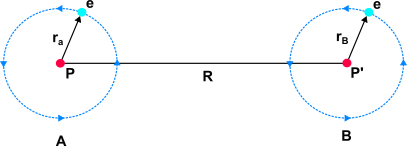
\includegraphics[width=0.48\textwidth]{waals} % Adjust width as needed
\end{wrapfigure}

Dato che i due atomi sono sono neutri, a grande distanza l'interazione Coulombiana risulta essere nulla, dato che due elementi a carica neutra non si attraggono o respingono. Essendo per\`o composti da  particelle di carica opposta questi possiedono un momento di dipolo elettrico non nullo
\begin{equation*}
	\bold{d}_{A} = e\bold{r}_{A} \quad \text{e} \quad \bold{d}_{B} = e\bold{r}_{B}
\end{equation*}
Un atomo che possiede un momento di dipolo genera un potenziale elettromagnetico rilevabile anche a grande distanza e quindi l'atomo A risente del campo magnetico di B e viceverso. Di conseguenza abbiamo un interazione elettrostatica tra i due dipoli:
\begin{equation*}
	\Delta \phi = \frac{\bold{d}_{A} \bold{d}_{B}}{R^3} - \frac{3(\bold{d}_{A} \cdot \bold{R})(\bold{d}_{B} \cdot \bold{R})}{R^5}
\end{equation*}
dove $|\bold{r}_{A}, \bold{r}_{B}| \ll R$. Da cui il potenziale d'interazione \`e 
\begin{equation}
	V = \frac{e^2}{R^3}[\bold{r}_{A} \cdot \bold{r}_{B} - 3 (\bold{r}_{A} \cdot \bold{n})(\bold{r}_{B} \cdot \bold{n})]
\end{equation}
con $\bold{n} = \bold{R}/\parallel \bold{R}\parallel $. Se ipotizziamo che $\bold{R}$  parallelo alla direzione $\hat{u}_{z} $ possiamo scrivere (5.38) nella seguente forma
\begin{equation*}
	V = \frac{e^2}{R^3}[x_{A}x_{B} + y_{A}y_{B} -2z_{A}z_{B}]
\end{equation*}
La Hamiltoniana che descrive la dinamica del sistema \`e duque data da 
\begin{equation*}
	H_0 = - \frac{\hbar^2}{2m}(\nabla_{A}^2 + \nabla_{B}^2) - \frac{e^2}{r_{A}} - \frac{e^2}{r_{B}}
\end{equation*}
che descrive il sistema imperturbato e la somma del potenziale d'interazione V
\begin{equation*}
	H = H_0 + V
\end{equation*}
Lo stato fondamentale per il sistema imperturbato $H_0$ \`e dato dal prodotto tensoriale degli stati fondamentali dei corrispettivi atomi A e B, ovvero
\begin{equation*}
	|0 \rangle  = |100 \rangle_{A} \otimes |100 \rangle_{B}
\end{equation*}
\newpage 
\subsection{Correzioni al primo ordine $\mathcal{O}(E)$ per lo stato fondamentale}

Per determinare le correzioni al primo ordine calcoliamo
\begin{equation*}
	 \langle 0 | V | 0 \rangle  = 0
\end{equation*}
e risulta essere nulla, in quanto per come abbiamo definito il potenziale V, i termini $\langle 100|x_A|100 \rangle,\ldots, ecc \ldots$ hanno come armonica sferica $Y_{00} = 1/\sqrt{4 \pi }$ e dato che i fattori di V sono funzioni dispari si ha per parit\`a che tutti gli elementi sono nulli.

\subsection{Correzioni al secondo ordine $\mathcal{O}(E)$ per lo stato fondamentale}
Le correzioni al secondo ordine sono date da 
\begin{equation*}
	E^{(2)} = \frac{e^4}{R^6} \sum_{\substack{nlm  \\[0.1cm]  n'l'm'}} \frac{|\langle nlm|_{A}\otimes \langle n'l'm'|_{B})V(|100 \rangle_{A} \otimes |100 \rangle_{B})|^2}{2E_1 -E_n - E_{n'}}
\end{equation*}
abbiamo che in generale la sommatoria restituisce un termine negativo, e quindi un energia negativa di conseguenza si ha una forza di natura attrattiva. Possiamo dunque riassumere che le forze di Van der Waals hanno un ordine di grandezza rispetto alla distanza di $\simeq 1 / R^6$ e sono un effetto al secondo ordine della teoria delle perturbazioni.

\section{Struttura fine dell'atomo d'idrogeno}

\subsection{Ripasso sull'atomo d'idrogeno}

Sappiamo che la Hamiltoniana di un atomo d'idrogeno in un sistema imperturbato \`e data da
\begin{equation*}
	H_0 = \frac{\bold{p}^2}{2m} - \frac{e^2}{r}
\end{equation*} 
di cui conosciamo sia autostati e autovalori associati, ovvero $|nlm \rangle$ e $E_n = -E_0/n^2$. La Hamiltoniana $H_0$ che descrive l'interazione elettrone-protone \`e non relativistica, ovvero non consideriamo velocit\`a prossime a quella della luce e l'energia cinetica \`e quella data dalla meccanica Newtoniana.

Nella descrizione dell'atomo d'idrogeno del modello di Bohr la quantizzazione della velocit\`a cattura gli ordini di grandezza con cui si splittano i livelli di energia, infatti se consideriamo la velocit\`a al livello fondamentale abbiamo che 
\begin{equation*}
	v_1 = \frac{e^2}{\hbar } \equiv \frac{q^2}{4\pi \varepsilon \hbar}
\end{equation*}
se vogliamo considerare le correzioni relativistiche introduciamo la grandezza 
\begin{equation*}
	\frac{v_1}{c} = \frac{e^2}{c \hbar} \equiv \frac{q^2}{4 \pi \varepsilon c \hbar} \equiv \alpha = \frac{1}{137}
\end{equation*}
e prende il nome di \textit{costante di struttura fine}. Mentre l'energia allo stato fondamentale 
\begin{equation*}
	\frac{e^2}{a_0} = \frac{me^2}{\hbar^2} = \frac{m \alpha^2 \hbar^2 c^2}{\hbar^2} = \alpha^2 mc^2
\end{equation*}
Tali risultati ci dicono che la scala di energia dell'idrogeno \`e di un fattore $\alpha^2$ pi\`u piccola dell'energia a riposo dell'elettrone. Tenendo conto delle correzioni relativistiche possiamo riscrivere i livelli energetico come 
\begin{equation}
	E_n = - \frac{1}{2}\alpha^2 mc^2 \frac{1}{n^2}
\end{equation}
Il momento angolare associato all'idrogeno \`e 
\begin{equation*}
	p \simeq \frac{\hbar}{a_0} = \frac{me^2}{\hbar} = \frac{e^2}{\hbar c}mc \quad \rightarrow \quad p \simeq \alpha(mc)
\end{equation*}

La degenerazione dello spettro dell'atomo d'idrogeno \`e data dalla relazione
\begin{equation*}
	n = N+l+1
\end{equation*}
dove $N \geq $ \`e un polinomio di grado r che compare nella funzione d'onda dove la dipendenza di r in prossimit\`a dell'origine viene eliminata. Il numero quantistico $l \geq 0$ rappresenta il momento angolare dello stato. Per ogni $n$ fissato, il valore di $l$ \`e compreso tra zero e $n-1$. Per ogni valore fissato di $l$ l'autovalore di $L_z$ \`e $m \hbar$ con m che varia tra $-l$ ed $l$:
\begin{align*}
	& n = 1,2,... \quad \quad l = 0,1, \ldots, n-1 \\[0.5cm]
	& m = -l,\ldots,l \quad \quad \text{\# stati di energia } E_n = \sum_{l=0}^{n-1}(2l+1) = n^2
\end{align*}  
Gli stati dell'idrogeno possono essere riassunti nel seguente diagramma 
\begin{figure}[!ht]
\vspace{0.1in}
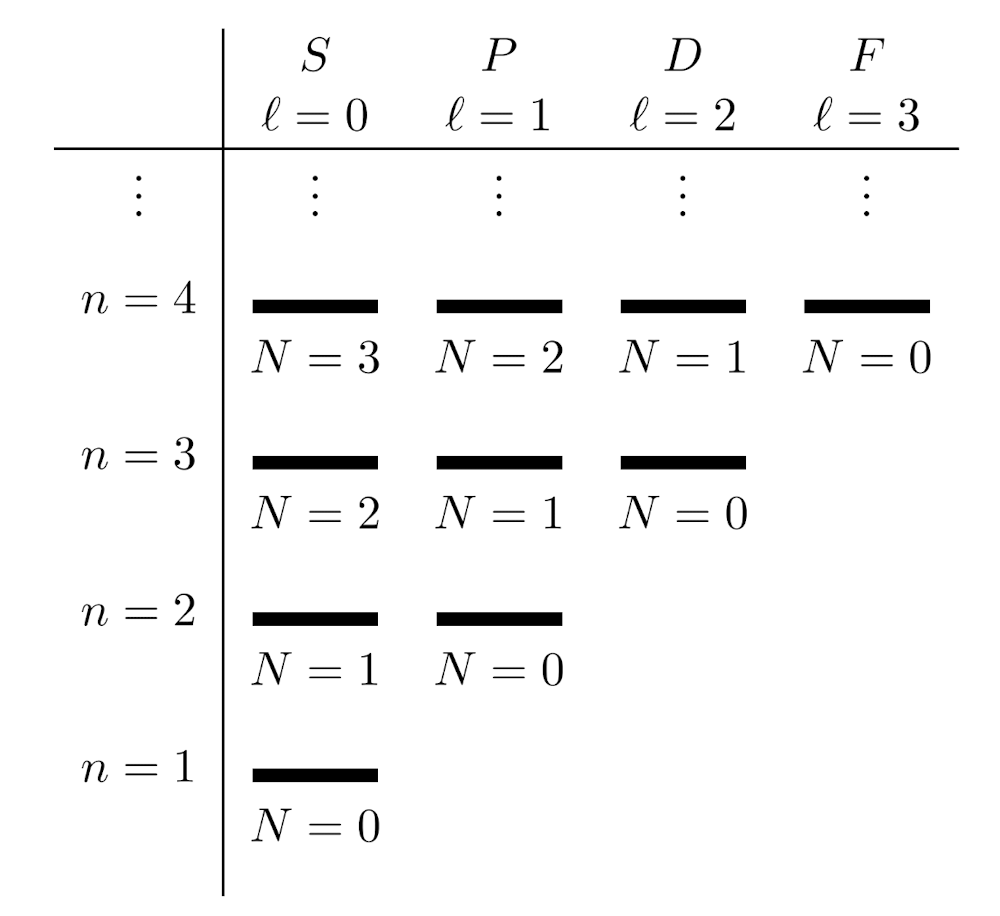
\includegraphics[width = 8cm]{hydrogen_states}	
\centering
\vspace{0.1in}
\end{figure}

Ogni autostato dell'atomo d'idrogeno \`e specificato dai tre numeri quantistici $n,l,m$ descritti dalle funzione d'onda
\begin{equation*}
	|nlm \rangle = A\left (\frac{r}{a_0}\right)^l \cdot \left ( \text{Polinomio in } \frac{r}{a_0}  \text{ di grado N}\right) \cdot e^{-r/na_0}Y_{l,m}(\theta ,\phi)
\end{equation*}
dove A \`e la costante di normalizzazione e $N = n - (l+1)$. Per lo stato fondamentale con $n=1,l=0$ e $m=0$ la funzione d'onda normalizzata \`e data da
\begin{equation*}
	|100 \rangle = \frac{1}{\sqrt{\pi a_0^3}}e^{-r/a_0}
\end{equation*}
Fino a questo punto nell'analisi di $H_0$ abbiamo ignorato lo spin dell'elettrone. Dato che un elettrone possiede spin $1/2$ \`e presente una degenerazione in pi\`u: ogni autostato di $H_0$ ha due stati di degenerazione, uno in cui si ha spin su e uno in cui si ha spin gi\`u. Questi stati sono degeneri perch\`e $H_0$ non ha termini dipendenza dallo spin.

Consideriamo due scelte differenti per la base degli stati dell'atomo d'idrogeno, entrambi che includono lo spin dell'elettrone.

Ricordiamo dalla trattazione dei momenti angolari accoppiati, che in generale per un momento $j$ accoppiato di due sistemi, abbiamo le coppie di stati $(j,m_j)$, dove $m_j$ varia da $-j$ a $j$ con incremento intero. Tutti gli stati composti sono autostati di $\bold{\hat{J}}^2$ con autovalori $\hbar^2j(j+1)$ e, per ogni stato, $\hbar m_j$ \`e l'autovalore di $\hat{J}_{z}$.

Dato che l'elettrone ha spin $1/2$ gli stati vengono indicati nel seguente modo
\begin{equation*}
	(s,m_s) \quad \text{con} \quad s=\frac{1}{2}, \quad m_{s} = \pm \frac{1}{2}
\end{equation*} 
Nell'atomo d'idrogeno il momento angolare $l$ pu\`o assumere diversi valori, ma lo spin dell'elettrone \`e sempre $1/2$. Per stati della base, questi sono descritti dai numeri quantici $n,l,m_l$ e $m_s$. Dato che non combiniamo lo spin dell'elettrone con il suo momento angolare, gli stati forma una base disaccoppiata
\begin{equation*}
	\mathcal{B} = \{|nlm_lm_s \rangle \} 
\end{equation*}
die elementi ortonormali tra loro.

Spesso \`e utile utilizzare una base alternativi dove gli stati sono autostati di $\hat{\bold{J}}^2$ e $\hat{J}_{z}$, dove il momento angolare totale $\bold{\hat{J}}$ \`e dato dalla somma del momento angolare orbitale $\bold{\hat{L}}$ e dallo spin della particella $\bold{\hat{S}}$:
\begin{equation*}
	\hat{\bold{J}} = \bold{\hat{L}} + \bold{\hat{S}}
\end{equation*}
Quando formiamo il prodotto tensoriale $l \otimes s$ stiamo considerando tutti i valori possibili di entrambi i numeri quantici. Tutti gli statti $l \otimes s$ sono autostati di $\hat{\bold{L}}^2$ e di $\bold{\hat{S}}^2$. Anche se gli stati non sono pi\`u autostati di $\hat{L}_{z}$ ed $\hat{S}_{z}$ lo sono ancora di $\hat{\bold{L}^2}$, quindi il numero quantistico $l$ sopravvive. La base accoppiata \`e descritta dai numeri quantici $(n,l,j,m_j)$.  I numeri $(m_l,m_s)$ della base disaccoppiata sono stati sostituiti da $(j,m_j)$. Gli stati accoppiati sono combinazione lineare di quelli disaccoppiati per cui si hanno differsi valori di $m_s$ e $m_l$, tali combinazioni restituisco lo stesso valore $m_j = m_l + m_s$.

Per determinare tutti gli stati accoppiati dobbiamo calcolare il prodotto tensoriale di ogni multicoppia $l$ dell'idrogeno con la coppia dello spin $1/2$. Le regole di addizione del momento angolare fanno si che il prodotto tensoriale assuma la forma
\begin{equation*}
	l \otimes \frac{1}{2} = \left (j=l + \frac{1}{2} \right ) \oplus \left (j = l-\frac{1}{2} \right )
\end{equation*}
PEr $l = 0$ otteniamo solo $j = 1/2$. Usando la notazione $L_j$ della tabella precedente con $L_j = S,P,D,F$ per $l = 0,1,2,3$. Il cambio della base \`e dato da 
\begin{equation*}
	l \otimes \frac{1}{2} \quad \rightarrow \quad L(l)_{j=l+ 1/2} \oplus L(l)_{j=l- 1/2}
\end{equation*}
o pi\`u esplicitamente
\begin{align*}
	& 0 \otimes 1/2 \quad \rightarrow \quad S_{1/2} \\[0.5cm]
	& 1 \otimes 1/2 \quad \rightarrow \quad P_{3/2} \oplus P_{1/2}\\[0.5cm]
	& 2 \otimes 1/2 \quad \rightarrow \quad D_{5/2} \oplus D_{3/2} \\[0.5cm]
	& 3 \otimes 1/2 \quad \rightarrow \quad F_{7/2} \oplus F_{5/2} 
\end{align*}
Usando questa notazione i multistati della base accoppiata, il diagramma dell'energia degli autostati dell'atomo d'idrogeno diventa 
\begin{figure}[!ht]
\vspace{0.1in}
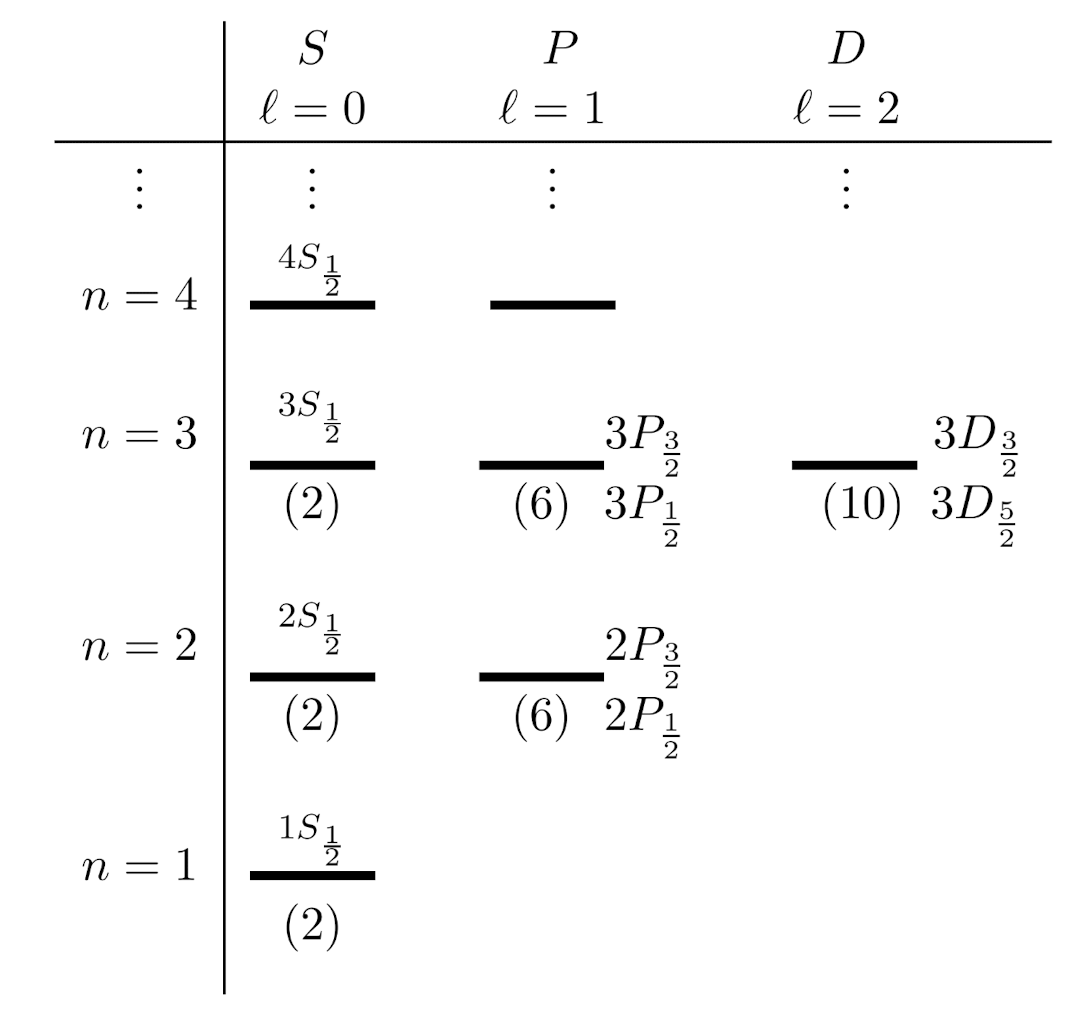
\includegraphics[width = 8cm]{coupled_hydrogen_basis}	
\centering
\caption{Il numero di stati per ogni livello \`e segnato in parentesi}
\vspace{0.1in}
\end{figure}
\subsection{L'equazione di Pauli}

Nell'atomo d'idrogeno l'accoppiamento tra spin e momento orbitale nasce dal fatto che l'elettrone di muove nel campo elettrico del protone. Dato che l'elettrone si muove relativamente al riferimento dove si ha il campo elettrico, nel riferimento dell'elettrone questo risulta essere soggetto ad un campo magnetico $\bold{B}$. L'accoppiamento tra spin-momento \`e dovuto all'interazione tra momento di dipolo magnetico dell'elettrone $\boldsymbol{\mu}$ e il campo magnetico $\bold{B}$, dato da $- \boldsymbol{\mu} \cdot \bold{B}$. In unit\`a di Gauss, il momento magnetico per una spira in un piano attraversata da una corrente I \`e data da $\boldsymbol{\mu} = \frac{I}{c}\bold{a}$, dove $\bold{a}$ \`e il vettore dell'area racchiusa dalla spira. Pert una particella di carica q e massa $m$, questa possiede momento magnetico equivalente a quello della spira e dunque 
\begin{equation*}
	\boldsymbol{\mu} = \frac{q}{2mc} \bold{L}
\end{equation*}
dove $\bold{L}$ \`e il momento angolare orbitale dovuto alla rotazione. Per una particella elementare, lo spin della particella e il momento magnetico si associano similmente al momento angolare, ma con un fattore di proporzionalit\`a $g$
\begin{equation*}
	\boldsymbol{\mu} = g \frac{q}{2mc}\hat{\bold{S}}
\end{equation*} 
dove $g = 2$ per un elettrone. Dato che $q = -e$, abbiamo che il momento di dipolo \`e dato da 
\begin{equation*}
	\boldsymbol{\mu} = 2 \frac{-e}{2m_ec}\hat{\bold{S}} = -2 \frac{e \hbar}{2m_ec}\frac{\hat{\bold{S}}}{\hbar} = -2 \frac{e \hbar}{2m_ec} \frac{1}{2}\boldsymbol{\sigma} = - \frac{e \hbar }{2m_ec}\boldsymbol{\sigma}
\end{equation*}
In termine numerici il fattore di proporzionalit\`a \`e il \textit{magnetone di Bohr} $\mu_B$ definito come
\begin{equation*}
	\mu_{B} = \frac{e \hbar}{2m_ec} \simeq 9.274 \times 10^{-21} \frac{erg}{gauss} = 5.79 \times 10^{-9} \frac{eV}{gauss}
\end{equation*} 
(nel sistema internazionale 1 Teslata = $10^4$ gauss). L'effetto di accoppiamento tra elettrone e campo magnetico esterno \`e quindi descritto dalla Hamiltoniana $H_B$ data da
\begin{equation*}
	H_B = - \boldsymbol{\mu} \cdot \bold{B} = \frac{e\hbar}{2m_ec}\boldsymbol{\sigma} \cdot \bold{B}
\end{equation*}
Ora vogliamo dimostra che l'accoppiamento, e il valore $g=2$, compaiono naturalmente dall'equazione non relativistica di Pauli per un elettrone.

Consideriamo l'equazione indipendente dal tempo di Schr\"odinger per una particella libera
\begin{equation*}
	\frac{\bold{p}^2}{2m}|\psi \rangle = E|\psi \rangle
\end{equation*}
Dato che una particella con spin $1/2$ ha due gradi di libert\`a, l'equazione precedente pu\`o essere espressa in forma vettoriale come
\begin{equation*}
	\frac{\bold{p}^2}{2m} \mathbb{I}_{2 \times 2} \chi = E \chi \quad \text{con} \quad \chi = \left [\begin{array}{c}
		\chi_1 \\ \chi_2
	\end{array}\right]
\end{equation*}
dove $\chi$ viene anche chiamato \textit{spinore di Pauli}. Possiamo riscrivere la Hamiltoniana usando le matrici di Pauli ricordando l'identit\`a
\begin{equation*}
	(\boldsymbol{\sigma} \cdot \bold{a})(\boldsymbol{\sigma} \cdot \bold{b}) = \bold{a} \cdot \bold{b} \; \mathbb{I}_{2 \times 2} + i \boldsymbol{\sigma} \cdot (\bold{a} \times \bold{b})
\end{equation*}
considerando $\bold{a} = \bold{p} = \bold{\hat{p}}$, dove $\hat{\bold{p}}$ \`e l'operatore momento, e dato che $\hat{\boldsymbol{p}} \times \bold{\hat{p}} = 0$ abbiamo che la relazione precedente diventa
\begin{equation*}
	(\boldsymbol{\sigma} \cdot \hat{\boldsymbol{p}})(\boldsymbol{\sigma} \cdot \hat{\boldsymbol{p}}) = \bold{\hat{p}^2} \;\mathbb{I}_{2 \times 2}
\end{equation*}
di conseguenza possiamo riscrivere la Hamiltoniana nel seguente modo
\begin{equation}
	H = \frac{1}{2m} (\boldsymbol{\sigma} \cdot \hat{\boldsymbol{p}})(\boldsymbol{\sigma} \cdot \hat{\boldsymbol{p}})
\end{equation}
Fino a questo punto ci siamo solo occupati di scrivere la fisica in un altra forma, ma nuovi fenomeni emergono quando accoppiamo una particella carica ad un campo elettromagnetico esterno. In meccanica quantistica per tenere conto dell'accoppiamento sostituiamo la quanti\`a di moto canonica con 
\begin{equation*}
	 \hat{\bold{p}} \quad \rightarrow \quad \hat{\boldsymbol{\pi}} \;  \equiv \hat{\bold{p}} - \frac{q}{c} \bold{A}
\end{equation*}
dove q \`e la carica della particella ed $\bold{A}$ il potenziale vettore, che \`e una funzione della posizione che diventa un operatore dato che la posizione \`e un operatore. Inoltre, se \`e presente un potenziale elettromagnetico scalare $\Phi$ questo contribuisce alla Hamiltoniana con un termine aggiuntivo $q \Phi(\bold{\hat{x}})$. 

Sostituendo in (5.40) abbiamo che e con i termini aggiuntivi otteniamo quella che viene definita \textit{Hamiltoniana di Pauli}
\begin{equation}
	H_{Pauli} = \frac{1}{2m}(\boldsymbol{\sigma} \cdot \hat{\boldsymbol{\pi}})(\boldsymbol{\sigma} \cdot \hat{\boldsymbol{\pi}})+q \Phi(\hat{\mathbf{x}}) .
\end{equation}
utilizzando l'identit\`a delle matrici di Pauli usata in precedenza il termine di prodotto vettoriale sopravvive e possiamo esprimerla esplicitamente come
\begin{equation*}
H_{\text {Pauli }}=\frac{1}{2 m}[(\hat{\boldsymbol{\pi}} \cdot \hat{\boldsymbol{\pi}}) \mathbb{1}+i \boldsymbol{\sigma} \cdot(\hat{\boldsymbol{\pi}} \times \hat{\boldsymbol{\pi}})]+q \Phi(\hat{\mathbf{x}}) .
\end{equation*}
Abbiamo che $\boldsymbol{\hat{\pi}}\times \boldsymbol{\hat{\pi}} \neq 0$ perch\`e le singole componenti non commutano tra loro. Infatti
\begin{equation*}
	(\hat{\boldsymbol{\pi}} \times \hat{\boldsymbol{\pi}})_k=\epsilon_{i j k} \hat{\pi}_i \hat{\pi}_j=\frac{1}{2} \epsilon_{i j k}\left[\hat{\pi}_i, \hat{\pi}_j\right] .
\end{equation*}
dove il commutatore \`e dato da
\begin{equation*}
	\left[\pi_i, \pi_j\right]=\left[p_i-\frac{q}{c} A_i, p_j-\frac{q}{c} A_j\right] 
\end{equation*}
Le componenti dell'operatore $\bold{\hat{p}}$ possono essere viste come delle derivate agenti sulle corrispettive componenti spazialmente dipendenti di $\bold{A}$. Inoltre le componenti $A_i$, essendo funzioni della posizione, commutano tra di loro.
\begin{equation*}
	[\pi_i , \pi_j] = - \frac{\hbar}{i}\frac{q}{c}(\partial_i A_j - \partial_j A_i) = \frac{i \hbar q}{c}(\partial_i A_j - \partial_j A_i)
\end{equation*}
Possiamo scrivere esplicitamente le componenti del prodotto vettoriale sostituendo il risultato orrenuto 
\begin{equation*}
	(\boldsymbol{\pi} \times \boldsymbol{\pi})_k=\frac{1}{2} \epsilon_{i j k} \frac{i \hbar q}{c}\left(\partial_i A_j-\partial_j A_i\right)=\frac{i \hbar q}{c} \epsilon_{i j k} \partial_i A_j=\frac{i \hbar q}{c}(\nabla \times A)_k
\end{equation*}
riassumibile come 
\begin{equation*}
	\boldsymbol{\hat{\pi}} \times \boldsymbol{\hat{\pi}} = \frac{i \hbar q}{c} \bold{B}
\end{equation*}
In conclusione la Hamiltoniana di Pauli diventa
\begin{equation*}
	H_{Pauli} = \frac{1}{2m} \left( \bold{\hat{p}} + \frac{e}{c} \bold{A} \right)^2 + \frac{e \hbar }{2mc} \boldsymbol{\sigma} \cdot \bold{B} - e \Phi(\bold{\hat{x}})
\end{equation*}
Il secondo termine nella Hamiltoniana di Pauli espansa fornisce informazioni sull'accoppiamento tra lo spin dell'elettrone e il campo magnetico come discusso ad inizio sezione.

\subsection{L'equazione di Dirac }

Anche se l'equazione di Pauli incorpora nella sua espressione l'accoppiamento tra lo spin dell'elettrone e il campo magnetico, non \`e un equazione relativistica. Per poter includere la relativit\`a al suo interno, bisogna modificare le matrici e lo spinore di Pauli, portandole ad uno spinore a quattro componenti. Questo \`e dovuto al fatto che nella teoria relativistica si deve tenere conto delle antiparticelle.

Iniziamo con l'analizzare le relazioni tra le energie e le quantit\`a di moto relativistiche
\begin{equation*}
	E^2 - \bold{p}^2c^2 = m^2c^4 \quad \rightarrow \quad E = \sqrt{\bold{p}^2c^2 + m^2 c^4}
\end{equation*}
Tale relazioni ci suggerisce che un Hamiltoniana che tiene conto di fattori relativistici per una particella libera debba essere espressa come
\begin{equation*}
	H = \sqrt{\bold{\hat{p}}^2c^2 + m^2 c^4}
\end{equation*}
la cui equazione di Schr\"odinger associata \`e data da
\begin{equation*}
	i \hbar \frac{\partial \psi }{\partial t} = \sqrt{\bold{\hat{p}}^2c^2 + m^2c^4} \psi
\end{equation*}
Ipotizziamo che $p \ll mc$, e quindi espandiamo la Hamiltoniana utilizzando Taylor
\begin{align*}
	H & = mc^2 \sqrt{1 + \frac{\bold{\hat{p}}^2}{m^2c^2}} = mc^2 \left [1 + \frac{\bold{\hat{p}}^2}{2m^2c^2} - \frac{1}{8} \left ( \frac{\bold{\hat{p}}^2}{m^2c^2}\right)^2 + \ldots \right] = \\[0.5cm]
	& = mc^2 + \frac{\bold{\hat{p}}}{2m} - \frac{1}{8}\frac{\bold{\hat{p}}^4}{m^3c^2} + \ldots
\end{align*}
Se si ignora la massa costante a riposo, il primo termine coincide con quello della Hamiltoniana non relativistica e quello successivo \`e una correzione relativistica. Per piccoli valori della quantit\`a di moto possiamo considerare il termine correttivo come una perturbazione.

Dirac voleva determinare una Hamiltoniana lineare rispetto ai momenti e privi di radici quadrate. Questo \`e possibile se si scrivono le energie relativistiche come quadrato di una funzione lineare rispetto ai momenti:
\begin{equation}
	c^2 \bold{\hat{p}}^2 + m^2 c^4 = (c \boldsymbol{\alpha} \cdot \bold{\hat{p}} + \beta mc^2)^2 = (c \alpha_1 \hat{p}_1 + c \alpha_2 \hat{p}_2 + c \alpha_3 \hat{p}_3 + \beta mc^2)^2
\end{equation} 
\newpage
Espandendo i termine di destra ed uguagliando i coefficienti si trova che le seguenti relazioni sono verficate
\begin{align*}
	& \alpha_1^2 = \alpha_2^2 = \alpha_3^2 = \beta^2 = 1 \\[0.1cm]
	& \alpha_i\alpha_j + \alpha_j\alpha_i = \{ \alpha_i , \alpha_j \} = 0 \quad i \neq j  \\[0.1cm]
	& \alpha_i \beta + \beta \alpha_i = \{\alpha_i,\beta\} = 0
\end{align*}
Le relazione alla seconda e terza riga ci dicono che $\alpha$ e $\beta$ non possono essere numeri, perch\`e devono essere nulle. Di conseguenza si ha che $\alpha$ e $\beta$ sono matrici hermitiane $2 \times 2$
\begin{equation*}
	\boldsymbol{\alpha} = \left [ \begin{array}{cc}
		0 & \boldsymbol{\sigma} \\ \boldsymbol{\sigma} & 0
	\end{array} \right]  
	,\quad 
	\beta =  \left [ \begin{array}{cc}
		\mathbb{I} & 0 \\ 0 & -\mathbb{I}
	\end{array} \right]  
\end{equation*}
Usando la relazione (5.42) la Hamiltoniana di Dirac coincide con la funzione lineare del momento che \`e la radice quadrata di $c^2 \bold{\hat{p}}^2 + m^2 c^4$. Dunque abbiamo che
\begin{equation*}
	H_{Dirac} = c \boldsymbol{\alpha} \cdot \bold{p} + \beta m c^2
\end{equation*}
L'equazione di Dirac associata \`e 
\begin{equation*}
	i \hbar \frac{\partial \Psi}{\partial t} = (c \boldsymbol{\alpha} \cdot \bold{p} + \beta m c^2) \Psi
\end{equation*}
dove $\Psi$ \`e lo \textit{spinore di Dirac}, che corrisponde a un vettore colonna costituito da quattro componenti che pu\`o essere visto come composizione di due spinori di Pauli $\chi$ e $\eta$ a due componenti
\begin{equation*}
	\Psi = \left [ \begin{array}{c}
		\chi \\ \eta 
	\end{array}\right]
	,\quad
	\chi = \left [ \begin{array}{c}
		\chi_1 \\ \chi_2 
	\end{array}\right]
	 ,\quad
	 \eta = \left [ \begin{array}{c}
		\eta_1 \\ \eta_2 
	\end{array}\right]
\end{equation*}
L'accoppiamento al campo elettromagnetico viene tenuto conto considerando la trasformazione definita nella sezione precedente e quindi abbiamo che l'equazione di Schr\"odinger diventa
\begin{equation*}
	i \hbar \frac{\partial \Psi}{\partial t} = \left [ c \boldsymbol{\alpha} \cdot \left ( \bold{\hat{p}} + \frac{e}{c}\bold{A}\right) + \beta mc^2 + V(r) \right]\Psi
\end{equation*}
dove l'accoppiamento dell'elettrone viene introdotto considerando un potenziale scalare $\Phi(r)$
\begin{equation*}
	V(r) = - e \Psi(r) =- \frac{e^2}{r}
\end{equation*}
Il grande vantaggio dell'equazione di Dirac \`e che le correzioni della Hamiltoniana $H_0$ dell'idrogeno possono essere derivate in modo sistematica trovando l'appropriata Hamiltoniana H che agisce sullo spinore di Pauli $\chi$. L'analisi pu\`o essere fatta considerando $\bold{A} = 0$, dato che la stazionariet\`a del protone non genere vettore potenziale. Il risultato dell'analisi dimostra che 
\begin{equation*}
	H \chi = E \chi
\end{equation*} 
dove 
\begin{equation}
	H = \underbrace{ \frac{\hat{\bold{p}}^2}{2m} + V}_{H_0} - \underbrace{\frac{\bold{\hat{p}}^4}{8m^3c^2}}_{\delta H_{rel}} + \underbrace{\frac{1}{2m^2c^2r} \frac{1}{r} \frac{dV}{dr} \bold{S} \cdot \bold{L}}_{\delta H_{spin-orbita}} + \underbrace{\frac{\hbar^2}{8m^2c^2}\nabla^2 V}_{\delta H_{Darwin}}
\end{equation}
Il primo termine correttivo corrisponde a quello dell'energia relativistica come visto in precedenza. Il secondo termine rappresenta l'accoppiamento spin-orbita ed infine abbiamo la correzione di \textit{Darwin}, che come vedremo interagisce solo lo stato $l = 0$.

Ricordiamo che la scala energetica per gli autostati di $H_0$ \`e data da $\alpha^2 mc^2$. Vedremo che tutte le correzioni per alti livelli di energia sono dell'ordine di $\alpha^4 m c^2$ mentre di un fattore $\alpha^2$ le pi\`u piccole. Questo ci suggerisce che per l'atomo d'idrogeno , il ruolo del parametro $\lambda$ della teoria delle perturbazioni \`e dato dalla costante di struttura fine $\lambda \sim \alpha^2$.

Per le correzioni relativistiche, dove $p \simeq \alpha mc $, abbiamo che il primo termine diventa 
\begin{equation*}
	\delta H_{rel} = - \frac{\bold{p}^4}{8m^3 c^2} \sim - \alpha^4mc^2
\end{equation*}
Per la componente spin-orbita, riscriviamo il termine
\begin{equation*}
	\frac{1}{r}\frac{dV}{dr} = \frac{1}{r} \frac{d}{dr} \left( -\frac{e^2}{r}\right) = \frac{e^2}{r^3}
\end{equation*}
e quindi
\begin{equation*}
	\delta H_{spin-orbita} = \frac{e^2}{2m^2c^2} \frac{1}{r^3} \bold{S} \cdot \bold{L}
\end{equation*}
Stimiamo il proddotto spin e momento orbitale come $\bold{S} \cdot \bold{L} \sim \hbar^2 $, $r \sim a_0$, dove $a_0 = \hbar / mc \alpha$ e corrisponde al raggio di Bohr:
\begin{equation*}
	\delta H_{spin-orbita} \sim \frac{e^2}{m^2c^2} \frac{\hbar^2}{a_0^3} = \frac{\alpha \hbar c}{m^2 c^2}\frac{\hbar^2}{a_0^3} = \alpha \left( \frac{\hbar}{mca_0} \right )^3 mc^2 = \alpha^4 mc^2
\end{equation*}
Possiamo valutare il termine di Darwin ponendo $V = - e^2/r$:
\begin{equation*}
	\delta H_{Darwin} = - \frac{e^2 \hbar^2}{8 m^2 c^2} \nabla^2 \left( \frac{1}{r}\right) = \frac{e^2 \hbar^2}{8 m^2 c^2}(-4 \pi \delta(\bold{r})) = \frac{\pi}{2} \frac{e^2 \hbar^2}{m^2 c^2}\delta(\bold{r})
\end{equation*}
Per stimare questo termine correttivo notiamo che data la funzione $\delta $, l'integrale del valore di aspettazione introduce un fattore $|\psi(\bold{0})|^2 \sim a_0^{-3}$, e quindi abbiamo che
\begin{equation*}
	\delta H_{Darwin} \sim \frac{e^2 \hbar^2}{m^2 c^2 a_0^3} \sim \alpha^4 mc^2
\end{equation*}
che coincide esattamente con la stessa combinazione di costanti che otteniamo per il termine correttivo spin-orbita.

\subsection{Calcolo delle correzioni delle energie}

La struttura fine dell'atomo di idrogeno \`e lo spettro dell'atomo che tiene in considerazione i termini correttivi determinati fino ad ora. Date le semplificazioni viste nella sezione precedente 
\newpage
abbiamo che il sistema \`e descritto dalla Hamiltoniana 
\begin{equation}
	H=\underbrace{\frac{\hat{\mathbf{p}}^2}{2 m}+V}_{H^{(0)}}-\underbrace{\frac{\hat{\mathbf{p}}^4}{8 m^3 c^2}}_{\delta H_{\text {rel}}}+\underbrace{\frac{e^2}{2 m^2 c^2} \frac{\mathbf{S} \cdot \mathbf{L}}{r^3}}_{\delta H_{\text {spin-orbita }}}+\underbrace{\frac{\pi}{2} \frac{e^2 \hbar^2}{m^2 c^2} \delta(\mathbf{r})}_{\delta H_{\text {Darwin }}} .
\end{equation}
in questa sezione studieremo ciascuno dei singoli termini  e combineremo i risultati per determinare la struttura fine dell'atomo d'idrogeno.

Consideriamo i livelli energetici $|n\;l\;m\;s \;m_s \rangle $ dove $s = 1/2$ e $m_s = \pm 1$. Per l'atomo d'idrogeno sono presenti livelli di energia degeneri, senza spin la degenerazione \`e dell'ordine $n^2$, ma introducendolo abbiamo una degenerazione di $2n^2$ e quindi lo stato fondamentale \`e degenere due volte.

Calcoliamo i termini correttivi al primo ordine dell'energia determinando le componenti della matrice perturbativa $2n^2 \times 2n^2$ date da
\begin{equation*}
	\langle n' \; l' \; m' \; s \; m_s' \mid V \mid n \; l \; m \; s \; m_s \rangle 
\end{equation*}
diagonalizzandola otteniamo gli autovalori che correggono l'energia.

Per semplificare i conti possiamo scegliere una base particolare data dalle costanti del moto del sistema. La Hamiltoniana del sistema imperturbato $H_0$ \`e ha come costanti del moto 
\begin{equation*}
	[L,H] = [S,H] = 0
\end{equation*}
Dato che H in riferimento al sistema perturbato contiene il termine $\bold{L} \cdot \bold{S}$, abbiamo che $\bold{L}$ e $\bold{S}$ non sono pi\`u costanti del moto.  La costante del moto diventa il momento angolare totale del sistema $\bold{J} = \bold{L}+ \bold{S}$ poich\`e
\begin{align*}
	& [\bold{L}^2,H] = 0 \quad \rightarrow \quad [\bold{L}^2,L_i] = 0 \\[0.2cm]
	& [\bold{S}^2,H] = 0 \quad \rightarrow \quad [\bold{S}^2,S_i] = 0 \\[0.2cm]
	& [\bold{J}^2,H] = 0 \\[0.2cm]
	& [\bold{J}_i,H] = 0 \quad \rightarrow \quad [J_i,\bold{J}^2] = 0  
\end{align*}
Le prime due righe ci dicono che $\bold{L} \cdot \bold{S}$ commuta con $\bold{L}^2$ e $\bold{S}^2$. Dall'ultimo termine possiamo definire 
\begin{equation*}
	\bold{L} \cdot \bold{S} = \frac{(\bold{S} + \bold{L})^2- \bold{S}^2 - \bold{L}^2}{2} = \frac{\bold{J}^2 - \bold{S}^2-\bold{L}^2}{2}
\end{equation*}
Le costanti del moto sono dunque date da $\{\bold{J}^2,\bold{L}^2,\bold{S}^2,J_i,H\}$ e questo ci suggerisce di passare ad una base in cui consideriamo il momento angolare 
\begin{equation*}
	|n \; l \; s \; j \; m_j \rangle 
\end{equation*}
L'utilizzo di osservabili compatibili, fa s\`i che possano essere diagonalizzate simultaneamente e in modo equivaalente gli autostati della Hamiltoniana si organizzano in modo da essere autostati di ciascun osservabile.
Se prendiamo un certo livello $n$ a cui \`e associato un determinatore valore $l$, avremo che 
\begin{equation*}
	m = -l,\ldots,l \quad \text{e per} \quad s = \frac{1}{2} \rightarrow m_s = \pm \frac{1}{2} \quad \Rightarrow \quad |l-s| \leq j \leq l+s 
\end{equation*}
Complessivamente abbiamo $2(2l+1)$ stati di split del livello energetico.
\vspace{1cm}
\begin{center}
\begin{tikzpicture}
	\draw[level] (0,0) -- node[above]{l $m_l = -l, \ldots,l$} node[below]{s $m_s = -1/2,1/2$} (5,0);
	\draw[level] (5,0) -- node[above]{} (6,0.5);
	\draw[level] (6,0.5) -- node[above]{$j = l + 1/2 \quad m_j = -j,\ldots,j $} (13,0.5);
	\draw[level] (5,0) -- node[]{} (6,-0.5);
	\draw[level] (6,-0.5) -- node[below]{$j = l - 1/2 \quad m_j = -j, \ldots, j$} (13,-0.5);
\end{tikzpicture}
\end{center}
Lo spin si combina aumentando o diminuendo il momento angolare di $\pm 1/2$ e ogni livello si suddivide in due. In generale uno stato \`e dato da 
\begin{equation*}
	|nlsjm_j \rangle = R_{nl}(r) \{\text{momento angolare + spin}\}
\end{equation*}
dunque bisogna prendere le armoniche sferiche e gli stati con gli spin $\uparrow \downarrow$ e fare le opportune combinazioni lineari, gli elementi della matrice di perturbazione dipenderanno dalla componente radiale degli autostati.

Consideriamo il primo termine corretivo dato da $\delta H_{rel}$ il contributo al termine matriciale sar\`a dato da 
\begin{align*}
	\langle \ldots \mid - \frac{\bold{p}^4}{8m^3c^4}\mid \ldots \rangle & = \langle \ldots \mid -\frac{1}{2mc^2}\left( \frac{\bold{p}^2}{2m}\right)^2 \mid \ldots \rangle  = \\[0.3cm]
	& = \langle \ldots \mid - \frac{1}{2mc^2} \left ( E_n + \frac{e^2}{r}\right)^2 \mid \ldots \rangle = \\[0.3cm]
	& = \delta_{jj'}\delta_{m_jm_{j'}}\delta_{ll'} \left( \frac{4n}{l + 1/2} -3\right)\left( - \frac{E_n}{2mc^2}\right)
\end{align*}
Per il secondo termine correttivo $\delta H_{spin-orbita}$ dato dall'accoppiamento spin-orbita abbiamo che 
\begin{align*}
	\langle \ldots \mid \frac{1}{2m^2c^2}\frac{e^2}{r^3} \bold{L} \cdot \bold{S}|\ldots \rangle & = \langle \ldots \mid \frac{1}{2m^2c^2}\frac{e^2}{r^3} \frac{\bold{J}^2 - \bold{L}^2 - \bold{S}^2}{2} |\ldots \rangle = \\[0.4cm]
	& = \frac{\hbar^2}{2}[j(j+1)-l(l+1)-s(s+1)]\langle \ldots \mid \frac{1}{2m^2c^2}\frac{e^2}{r^3} \mid \ldots \rangle = \\[0.4cm]
	& = \frac{E_n^2}{mc^2} \frac{n(j(j+1)-l(l+1)-s(s+1)}{l(l+1)(l+1/2)}\delta_{jj'}\delta_{ll'}\delta_{m_j m_{j'}}
\end{align*}
Infine il terzo termine correttivo dato da $\delta H_{Darwin}$ ci restituisce un contributo all'elemento matriciale 
\begin{equation*}
	\langle \ldots | \frac{\hbar^2}{8 m^2 c^2}4 \pi e^2 \delta(\bold{r}) \mid \ldots \rangle = \frac{E_n^2}{mc^2}2n \delta_{jj'}\delta_{ll'}\delta_{m_j m_{j'}} \delta_{l0} 
\end{equation*}
dove il termine $\delta_{l0}$ \`e dovuto al fatto che si valuta la funzione in $\bold{r} = 0$, di conseguenza il contributo \`e non nullo solo per $l=0$ e quindi per $j = 1/2$.


Tutti i termini trovati sono diagonali rispetto alla base del momento angolare totale $\bold{J}$. Per l'atomo d'idrogeno i termini si combinano in modo tale che l'energia complessiva dipenda solo da $j$ e non da $l$. La formula per un livello di energia \`e 
\begin{equation}
	E_{nj} = - \frac{E_0}{n^2} \left[1 + \frac{\alpha^2}{n^2}\left(\frac{n}{j + 1/2} - \frac{3}{4} \right) \right]
\end{equation}
che corrisponde ad una correzione dell'ordine di $\alpha^2$ dei livelli energetici.

L'equazione di Dirac ammette soluzione esatta e la formula esatta degli autostati energetici \`e data da 
\begin{equation*}
	E_{nj} = mc^2 \left \{ \left [ 1 + \left( \frac{\alpha}{n-(j+1/2) + \sqrt{(j+1/2)^2-\alpha^2}}\right)^2\right]^{-1/2}-1 \right \}
\end{equation*}

\subsubsection{Esempio}
 Consideriamo il livello fondamentale per $n=1,l=0,j =1/2$ e $m_j = \pm 1/2$ si ha degenerazione, ovvero il livello energetico si splitta in due 
 \vspace{1cm}
\begin{center}
\begin{tikzpicture}
	\draw[level] (0,0) -- node[above]{$1S$}  (5,0);
	\draw[level] (5,0) -- node[above]{} (6,0.5);
	\draw[level] (6,0.5) -- node[above]{$j = 1/2  $} (13,0.5) node[right]{$1S_{1/2}$};
	\draw[level] (5,0) -- node[]{} (6,-0.5);
	\draw[level] (6,-0.5) -- node[below]{$j =  -1/2 $} (13,-0.5) node[right]{$1S_{-1/2}$};
\end{tikzpicture}
\end{center}
 Se consideriamo invece $n=2$ avremo due valori possibili del momento angolare $l = 0 ,1$ che in notazione spettroscopica sono i livelli $2S$ e $2P$. Per il livello 2s abbiamo che questo coincide con il livello $1S_{1/2}$, ottenendo una degenerazione in due livelli energetici. Per il caso $2P$ abbiamo una degenerazione di sei livelli energetici dato che per $l =1$ e $s = 1/2$ si ha $j = 1/2 , 3/2$, di conseguenza il livello 2P si spezza  in due a seconda del valore del momento 
 \vspace{1cm}
\begin{center}
\begin{tikzpicture}
	\draw[level] (0,0) -- node[above]{$2P$}  (5,0);
	\draw[level] (5,0) -- node[above]{} (6,0.5);
	\draw[level] (6,0.5) -- node[above]{$j = 3/2  $} (13,0.5) node[right]{$2P_{3/2}$};
	\draw[level] (5,0) -- node[]{} (6,-0.5);
	\draw[level] (6,-0.5) -- node[below]{$j =  1/2 $} (13,-0.5) node[right]{$2P_{1/2}$};
\end{tikzpicture}
\end{center} 
a loro volta il livello energetico $2P_{3/2}$ si divide in altri quattro livelli di energia dato che $m_j = -3/2,-1/2,1/2,3/2$, mentre $2P_{1/2}$ in altri due dato che $m_j = - 1/2,1/2$.

Che graficamente possiamo rappresentare come 
\newpage

\vspace{1cm}
\begin{center}
\begin{tikzpicture}
	\draw[level] (0,0) -- node[above]{$2P$}  (3,0);
	\draw[level] (3,0) -- node[above]{} (4,0.5);
	\draw[level] (4,0.5) -- node[above]{$2P_{3/2}$}(6,0.5) ;
	\draw[level] (6,0.5) -- node[right]{}(7.5,1.5);
	\draw[level] (7.5,1.5) -- (9.5,1.5)node[right]{$m_j = 3/2$};
	\draw[level] (6,0.5) -- (7.5,1);
	\draw[level] (7.5,1) -- (9.5,1) node[right]{$m_j = 1/2$};
	\draw[level] (6,0.5) -- node[right]{}(7.5,-0.5);
	\draw[level] (7.5,-0.5) -- (9.5,-0.5)node[right]{$m_j = -3/2$};
	\draw[level] (6,0.5) -- (7.5,-0.);
	\draw[level] (7.5,-0.) -- (9.5,0.) node[right]{$m_j = - 1/2 $};
	\draw[level] (3,0) -- node[]{} (4,-2);
	\draw[level] (4,-2) -- node[below]{$2P_{1/2}$} (6,-2) ;
	\draw[level] (6,-2) -- (8,-1.5);
	\draw[level] (8,-1.5) -- (9.5,-1.5) node[right]{$m_j = 1/2$};
	\draw[level] (6,-2) -- (8,-2.8);
	\draw[level] (8,-2.8) -- (9.5,-2.8) node[right]{$m_j = - 1/2$};
\end{tikzpicture}
\end{center} 
La struttura fine separa i livelli energetici dell'atomo d'idrogeno, ma li lascia degeneri. La degenerazione \`e dovuta al fatto che il numero quantico $m_j$ essendo la proiezione del momento angolare in una direzione, fino a quando non viene rotta la simmetria sferica del problema, questo viene conservato. 

Il modulo del momento pu\`o essere arbitrario, ma la proiezione nello spazio \`e rilevante e l'assenza di $m_j$ nell'equazione dell'energia \`e spiegata dall'invarianza per rotazioni del problema.

\section{Teoria delle perturbazioni dipendenti dal tempo }

 
